

\begin{enumerate}[label = \arabic*)]
    \item Let X and Y be independent and identically distributed normal random variables. Then the characteristic function of X and Y is given by
    \begin{equation}
        \Phi_X(\omega) = e^{j\eta\omega - \sigma^2\omega^2/2}
    \end{equation}
    The characteristic function of Z is given by
    \begin{align}
        \Phi_Z(\omega) &= \Phi_X^2(\omega)\\
                       &= e^{2j\eta\omega - \sigma^2\omega^2}
    \end{align}
    Thus Z is a normal random variable with parameters $2\eta$ and $2\sigma^2$. Thus option (1) is correct.
    \item Let X and Y be independent and identically distributed exponential random variables. Then the characteristic function of X and Y is given by
    \begin{equation}
        \Phi_X(\omega) = \dfrac{\lambda}{1-j\omega}
    \end{equation}
    The characteristic function of Z is given by
    \begin{align}
        \Phi_Z(\omega) &= \Phi_X^2(\omega)\\
                       &= \dfrac{\lambda^2}{(1-j\omega)^2}
    \end{align}
    Thus Z is not an exponential random variable. Therefore option (2) is wrong.
    \item Let X and Y be independent and identically distributed uniform random variables such that X, Y $\sim$ U(a,b). Then the characteristic function of X and Y is given by
    \begin{equation}
        \Phi_X(\omega) = \dfrac{e^{jb\omega} - e^{ja\omega}}{j\omega(b-a)}
    \end{equation}
    The characteristic function of Z is given by
    \begin{align}
        \Phi_Z(\omega) &= \Phi_X^2(\omega)\\
                       &= -\dfrac{(e^{jb\omega} - e^{ja\omega})^2}{\omega^2(b-a)^2}
    \end{align}
    Thus Z is not a uniform random variable. Thus option (3) is wrong.
    \item Let X and Y be independent and identically distributed binomial random variables. Then the characteristic function of X and Y is given by
    \begin{equation}
        \Phi_X(\omega) = (pe^{j\omega}+q)^n
    \end{equation}
    The characteristic function of Z is given by
    \begin{align}
        \Phi_Z(\omega) &= \Phi_X^2(\omega)\\
                       &= (pe^{j\omega}+q)^{2n}
    \end{align}
    Thus Z is a binomial random variable with parameter 2n. Thus option (4) is correct.
\end{enumerate}
The following figures show the experimental distributions for Z in each case. The simulation length was kept one million.
\begin{figure}[!ht]
\centering
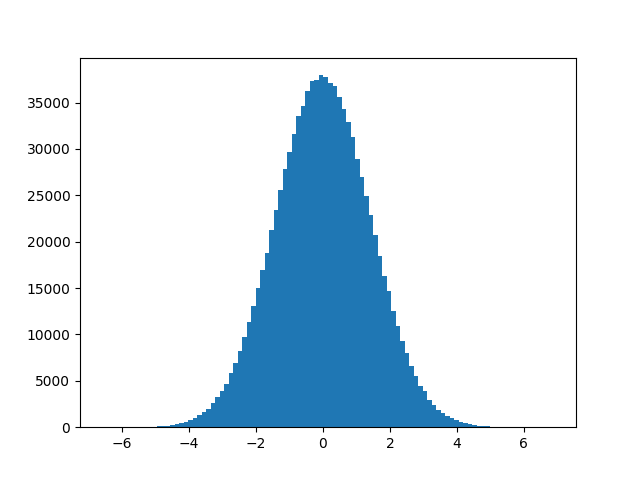
\includegraphics[width=\columnwidth]{solutions/2016/june/107/figures/norm.png}
\caption{Z when X is standard normal}
\label{june2016-107:fig:normal}
\end{figure}
\begin{figure}[!ht]
\centering
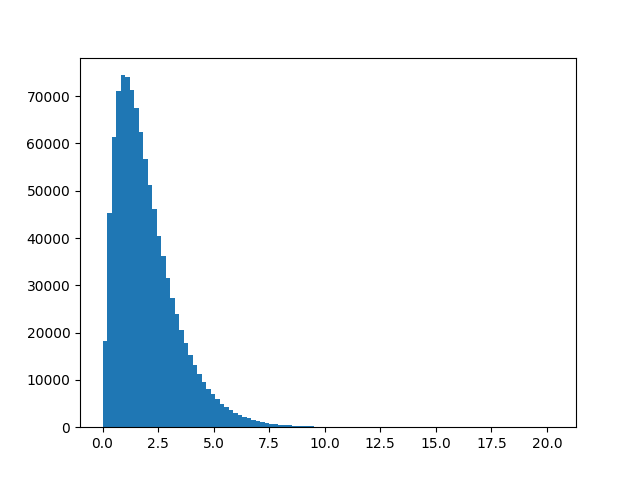
\includegraphics[width=\columnwidth]{solutions/2016/june/107/figures/expon.png}
\caption{Z when X is exponential with $\lambda = 1$}
\label{june2016-107:fig:exponential}
\end{figure}
\begin{figure}[!ht]
\centering
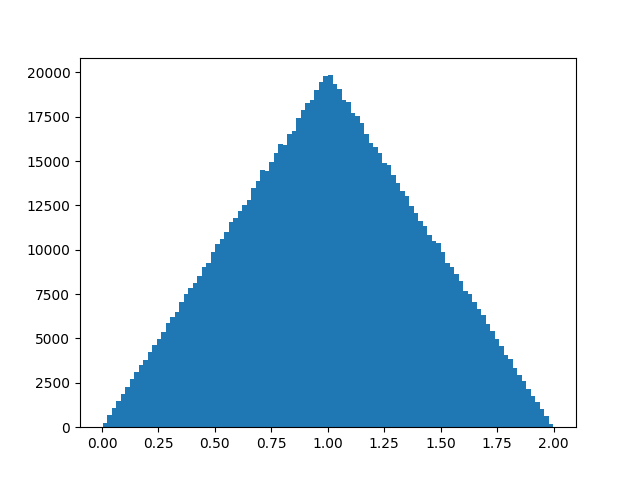
\includegraphics[width=\columnwidth]{solutions/2016/june/107/figures/uniform.png}
\caption{Z when X $\sim$ U(0,1)}
\label{june2016-107:fig:uniform}
\end{figure}
\begin{figure}[!ht]
\centering
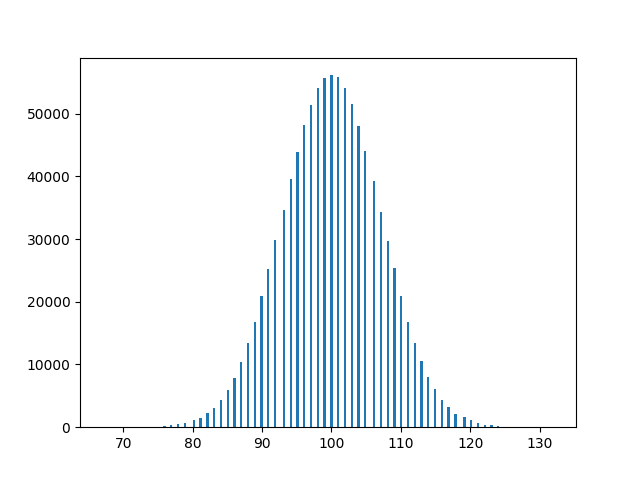
\includegraphics[width=\columnwidth]{solutions/2016/june/107/figures/binom.png}
\caption{Z when X $\sim$ B(100,0.5)}
\label{june2016-107:fig:binomial}
\end{figure}

